\documentclass{article}
\usepackage[utf8]{inputenc}
\usepackage[german]{babel}
\usepackage{amsmath}
\usepackage{amsfonts}
\usepackage{amssymb}
\usepackage{graphicx}
\usepackage[left=2cm,right=3cm,top=2cm,bottom=2cm]{geometry}

\title{Pflichtenheft}

\setlength{\parskip}{5mm plus4mm minus3mm}

\begin{document}

\maketitle
\newpage
\tableofcontents
\newpage

\section{Ausgangssituation und Zielsetzung}
Im Rahmen des Sommersemesterbeleges 2014 im Fach Software Engeneering II der Hochschule für Technik und Wirtschaft Dresden soll ein Softwaresystem zur vereinfachten Erfassung und Verwaltung von Beleggruppen unter Frau Professorin Hauptmann, weiterhin als Auftraggeberin benannt, erstellt werden.
Folgende Aufgabenstellung ist dabei zu realisieren:
Entwickeln  Sie ein SW-System, das die Verwaltung der Daten für Belegarbeiten, die auch parallel laufen können. Neben der Erfassung sind auch weitere Anwendungsfälle wie zum Beispiel „archivieren von Daten“ zu realisieren.
Dazu wird im folgendem die Aufgabenstellung auf 2 Programme aufgeteilt, Eines für die Studenten zum Anmelden und Verwalten ihrer eigenen Gruppe und zum anderen ein Programm für den Dozenten , welcher neben administrativer Funktionen auch Verwaltungsrelevante bekommt.

\section{Systemeinsatz, Systemumgebung}
\subsection{Anwendungsbereiche}
Das System wird zur Verwaltung von Beleggruppen unter dem Auftraggeber eingesetzt. Daher sind einige Festlegungen wie z.B.: die Caseanzahl ausdrücklich vom Auftraggeber festgelegt.
Das System soll als Client-Server Architektur realisiert werden. Der Datenbankserver wird dabei vom Auftraggeber gestellt und unterliegt daher weiterführend keiner genaueren Betrachtung. Zu Implementieren seien daher:
\begin{itemize}
\item Ein Programm damit Studentengruppen eine Gruppe erstellen und verwalten können
\item Ein Programm für den Dozenten mit erweiterten Funktionen hinsichtlich administrativer und verwaltungsrelevanter Aufgaben
\item Verwaltungsstruktur auf dem Datenbankserver um Informationen langfristig zu speichern
\end{itemize}
\subsection{Zielgruppe}
Das Softwaresystem wird zum einen von Studenten benutzt, welche unter dem Auftraggeber eine Belegarbeit anzufertigen haben und sich dazu in Gruppen einfinden und organisieren müssen.
Des Weiteren wird das System vom Auftraggeber sowie von Ihr festgelegten weiteren Berechtigten genutzt werden um die Studenten bei der Verwaltung ihrer Gruppe zu unterstützen sowie selbst eine einfachere Verwaltung von Belegarbeiten zu erhalten.
\subsection{Systemumgebung}
Das Softwaresystem kann nur im Intranet der Hochschule für Technik und Wirtschaft Dresden benutzt werden. 

\section{Benutzerschnittstellen}
\subsection{Client für Studenten}

\begin{center}
    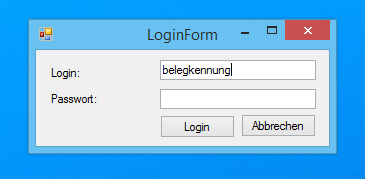
\includegraphics[scale=1]{bilder/pic3.PNG}\\
    Erstanmeldung für Studenten \\

    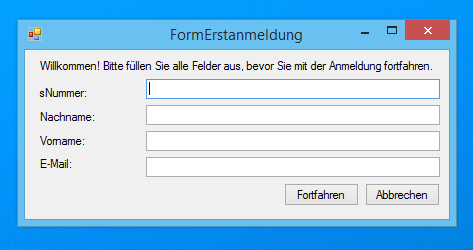
\includegraphics{bilder/pic4.PNG}\\
    Eingabe der persönlichen Informationen des Gruppenleiters \\
    
   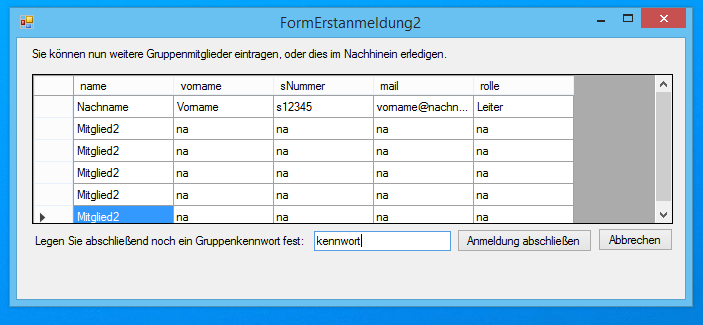
\includegraphics[scale=0.8]{bilder/pic6.PNG}\\
    Gruppenmitglieder werden automatisch in der gegebenen Mindestanzahl erstellt und können bearbeitet werden. Weiter erst nach Eingbabe eines Gruppenpassworts. \\
    
    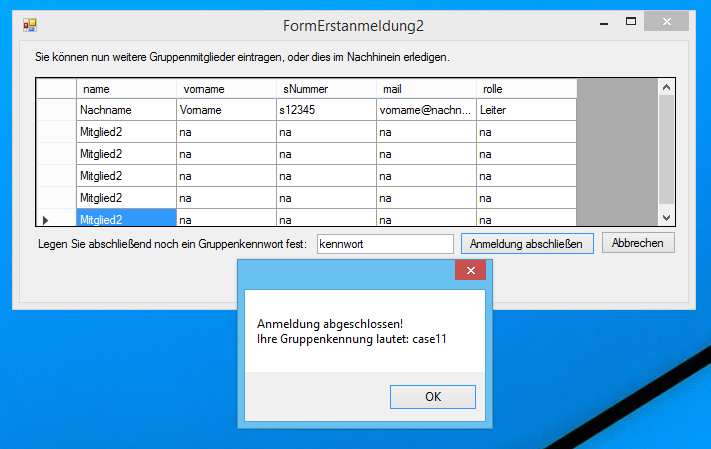
\includegraphics[scale=0.8]{bilder/pic7.PNG}\\
    Ist die Erstanmeldung erfolgreich abgeschlossen, wird vom System eine caseXX-Nummer zugeteilt, die die Gruppe in Zukunft als Gruppen-Login verwendet. \\
    
    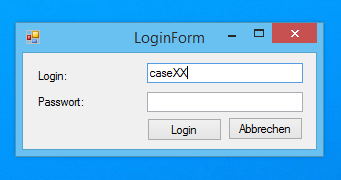
\includegraphics{bilder/pic2.PNG}\\
    Anmeldung für Studenten, wenn schon eine Gruppe existiert \\
    
    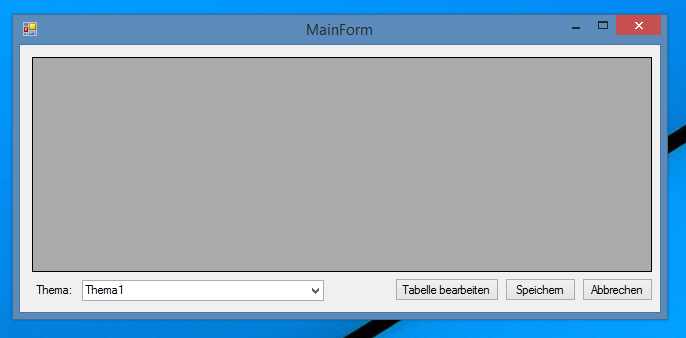
\includegraphics[scale=0.8]{bilder/pic8.PNG}\\
    Eigene Gruppe verwalten (Mitglieder ändern, Thema ändern) \\
\end{center}

\subsection{Client für Dozenten}
\begin{center}
    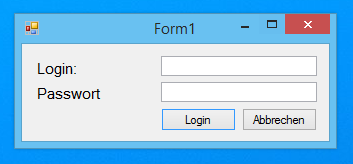
\includegraphics{bilder/doz1.PNG}\\
    Anmeldung für Dozenten \\
    
    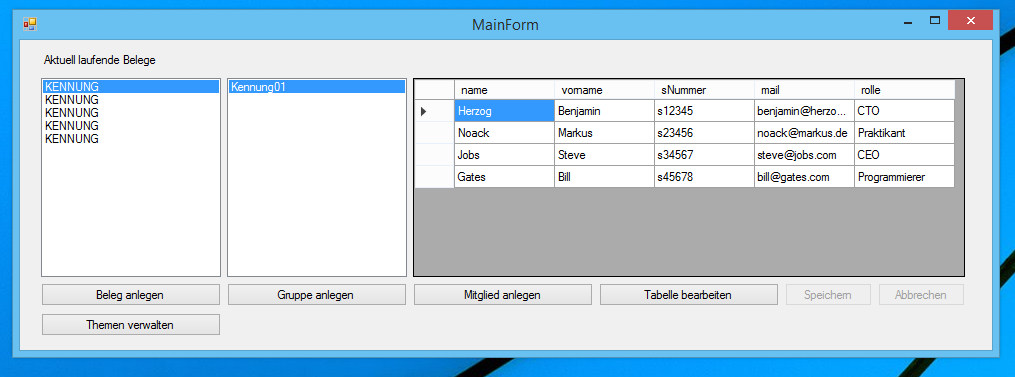
\includegraphics[scale=0.6]{bilder/doz2.PNG}\\
    Übersicht über alle Belege, dessen Gruppen und dessen Mitglieder direkt nach Anmeldung \\
    
    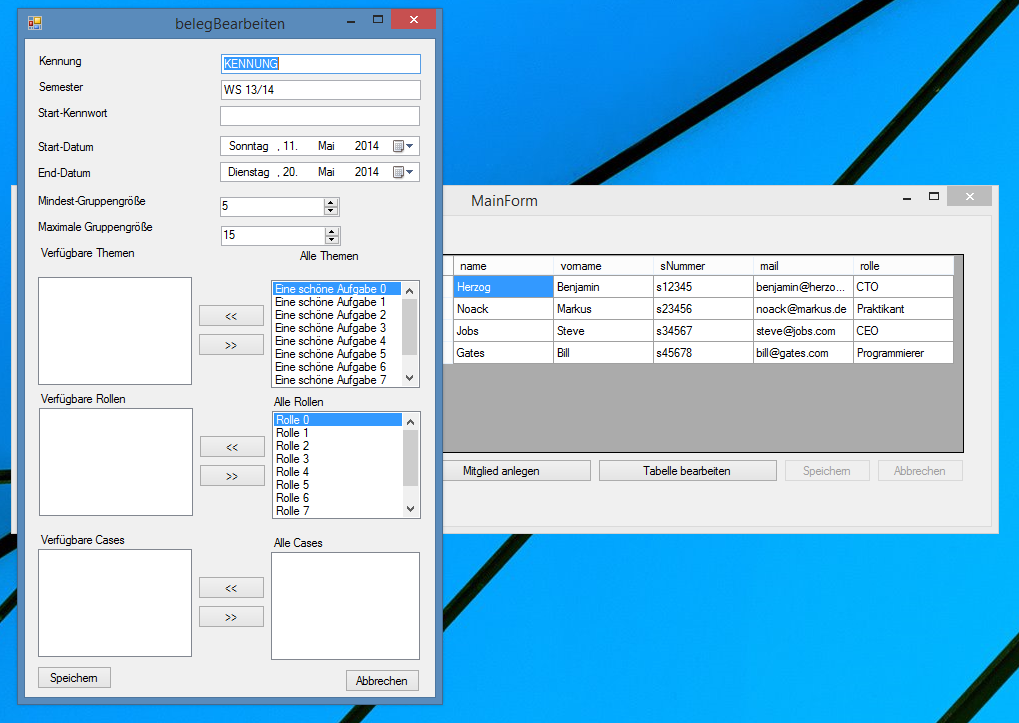
\includegraphics[scale=0.55]{bilder/doz3.PNG}\\
    Anlegen eines neuen Belegs mit den dazugehörigen Angaben \\
    
    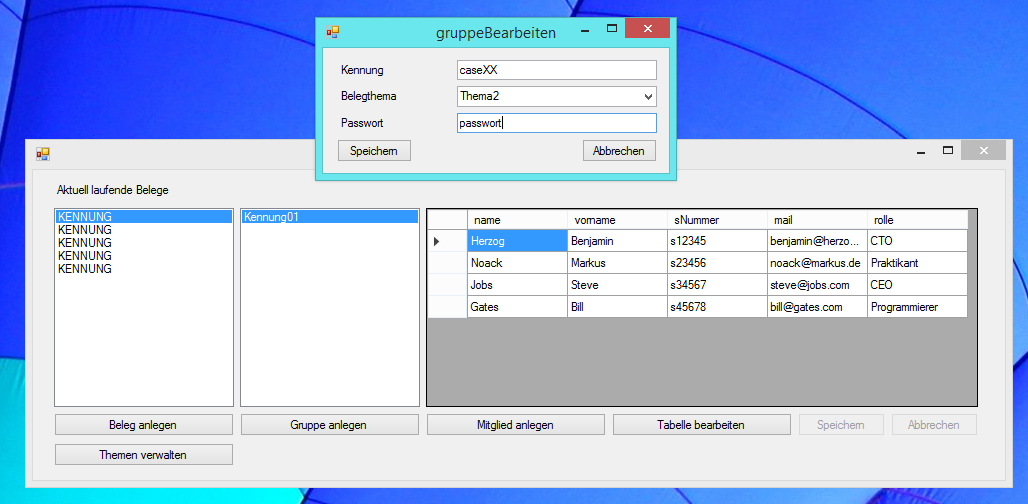
\includegraphics[scale=0.6]{bilder/doz4.PNG}\\
    Gruppe bearbeiten/anlegen, falls Studenten Zugangsdaten oder änhliches vergessen haben \\
    
    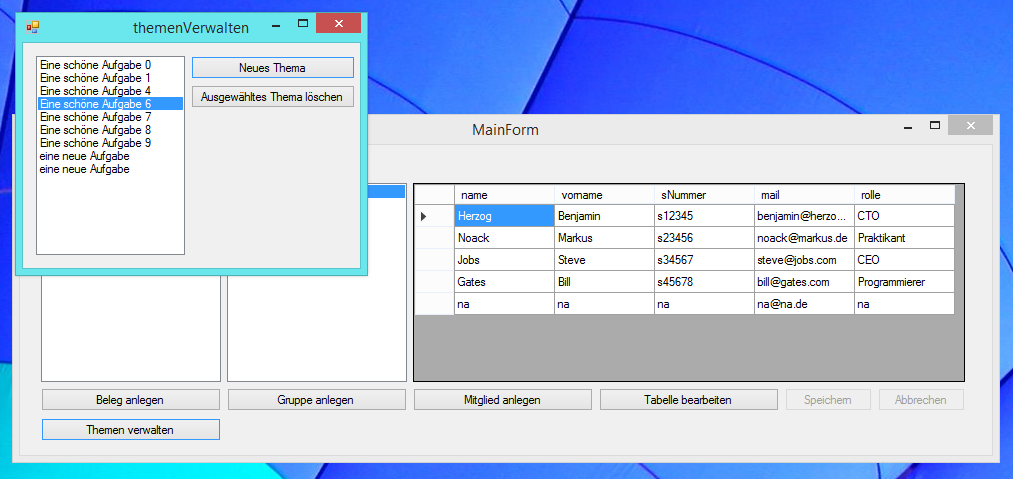
\includegraphics[scale=0.6]{bilder/doz5.PNG}\\
    Themen verwalten (anlegen/löschen) \\
\end{center}

\section{Funktionale Anforderungen}
Das Softwaresystem besteht aus mehreren Programmen, welche die Nutzung als Dozent oder als Projektgruppe erlaubt.\\\\

Dabei soll das Teilsystem des Dozenten eine hierarchische Auswahl der Auflistung der Belege, der Gruppen und der Daten der Gruppenmitglieder, sowie die Möglichkeit der Bearbeitung derselben enthalten.\\
Außerdem soll es die Erstellung neuer Belege und die Zuteilung von Gruppenslots(Cases) ermöglichen.\\
Dazu soll auch eine Zuteilung von Themen und Rollen aus jeweilig bearbeitbaren Pools zu einem Beleg möglich sein.\\
Weiterhin soll die Generierung einer PDF-Datei zur analogen Archivierung der im System enthaltenen Daten ermöglicht werden.\\
Als weiteres Feature soll dieses Teilsystem die durch spezifizierbare Kriterien bestimmte Datensätzen ausgeben, was grundlegend als Suchfunktion oder zur Generierung von E-Mail-Addresslisten genutzt werden kann.\\\\

Das Teilsystem, welches potenziellen Projektgruppen zur Verfügung gestellt werden wird, soll eine Loginfunktion zur näheren Spezifikation der Projektgruppe enthalten.\\
Dabei wird es neben Gruppennamen nach dem Schema "caseXX" ermöglicht, durch Eingabe einer Belegkennung und zugehöriger Passphrase eine neue Projektgruppe zu erstellen und einen entsprechenden Slot zugeteilt zu bekommen.\\
Nach erfolgreichem Login wird einerseits über bisherige Daten der eigenen Gruppe informiert, andererseits die Bearbeitung derselben ermöglicht.\\

Optional kann das Dozentenrelease eine Schnittstelle zu Mozilla Thunderbird beinhalten.\\
Ebenso optional kann es außerdem die Bereitstellung eines druckbaren Formulars zur Mitschrift der Benotung während oder nach der Präsentation eines Beleges enthalten.\\
%\begin{itemize}
%\item Login mit verschiedenen Berechtigungen(Projektgruppe/Dozent)
%\item hierarchische Auswahl der Auflistung der Belege, der Gruppen, der Daten
%der Gruppenmitglieder für Dozenten
%item Erstellung neuer Belege \& Zuteilung einer Anzahl an Gruppenslots(Cases)
%\begin{itemize}
%\item Zuteilung von Themen und dem Beleg aus einem bearbeitbaren Themenpool durch Dozent
%\item Zuteilung von Rollen und dem Beleg aus einem bearbeitbaren Rollenpool durch Dozent
%\end{itemize}
%\item lesender/schreibender Zugriff des Dozenten auf sämtliche Daten
%\item Generierung einer PDF-Datei mit entsprechenden Daten des Beleges
%\item Ausgabe von Datensätzen nach Erfüllung einstellbarer Kriterien(Namen,
%Rollenverteilung)
%\begin{itemize}
%\item relevant für Suchfunktionen und Generierung von E-Mail-Addresslisten
%\end{itemize}
%\end{itemize}
%\begin{itemize}
%\item Erstellung neuer Gruppen auf Basis eines vorgegebenen Beleg-Erstlogins
%\item tabellarische Auflistung der Gruppendaten aus Gruppenperspektive
%\item Änderungsfunktionen der Gruppendaten aus Gruppenperspektive
%\end{itemize}

%Optional:
%\begin{itemize}
%\item Thunderbird-Schnittschnelle(direktes öffnen)
%\item druckbares Formular zur Benotung
%\end{itemize}

\section{Qualitätsanforderungen}
\begin{itemize}
\item Benutzerfreundlichkeit (wird über Prototyp geregelt)
\item Zuverlässigkeit (Überprüfung von potentiellen Fehleingaben des Nutzers)
\item Sicherheit und Datenschutz (Gruppen durch Passwort geschützt)
\end{itemize}

\section{Rahmenbedingungen}
\begin{itemize}
\item Nutzung des hochschuleigenen Sybase-Servers
\item Die Datenbank (Sybase-DB) zum Speichern der Daten ist bereits vorhanden
(organisatorisch)
\item Anmeldung der Gruppe über einzelnes Login
\item Das Betriebssystem, auf dem das Softwaresystem hauptsächlich lauffähig
sein soll, ist Windows 7(technisch)
\item Gefordert ist eine Desktopanwendung (keine Webanwendung) (technisch)
\item Ein Thema darf von mehreren Gruppen bearbeitet werden (organisatorisch)
\item Beleggruppe darf innerhalb des Anmeldezeitraums flexibel mit Thema und Verantwortlichkeiten (Rollen) umgehen
\item Für das Speichern der Benutzerdaten (z.B. der Email-Adressen) gilt das
Datenschutzgesetz (rechtlich)
\end{itemize}

\section{Fehlertoleranzmaßnahmen}

\subsection{Generell}
\begin{tabular}{|p{7cm}|p{7cm}|}
\hline
	\textbf{Fehler}												&	\textbf{Reaktion / Gegenmaßnahme}						\\
\hline
\hline
	Verbindung Datenbank schlägt Fehl							&	Fehlermeldung anzeigen, erneut versuchen oder beenden	\\
\hline
	fehlerhafte Eingabe in Datums- und Zahlenfelder				&	die Eingabe falscher Zeichen in ein Eingabefeld wird von den verwendeten Komponenten verhindert	\\
\hline
	Anfragen an die Datenbank unter Umgehung des SW-Systems		&	Enge Berechtigungsvergabe und Prüfung der Eingabe auf Seite der Datenbank \\
\hline
\end{tabular}

\subsection{Gruppe erstellen}
\begin{tabular}{|p{7cm}|p{7cm}|}
\hline
	\textbf{Fehler}					&	\textbf{Reaktion / Gegenmaßnahme}									\\
\hline
\hline
	falsche Zugangsdaten eingegeben	&	Fehlermeldung anzeigen, Verzögerung in Datenbank, erneut versuchen	\\
\hline
	maximale Gruppenanzahl erreicht	&	Fehlermeldung, abbrechen											\\
\hline
\end{tabular}

\subsection{Gruppe bearbeiten}
\begin{tabular}{|p{7cm}|p{7cm}|}
\hline
	\textbf{Fehler}										&	\textbf{Reaktion / Gegenmaßnahme}				\\
\hline
\hline
	außerhalb des Anmeldezeitraumes						&	Benutzung des Buttons nicht möglich				\\
\hline
	Anzahl der Gruppenmitglieder unterschreitet minimum	&	Fehlermeldung, bearbeiten wird fortgesetzt		\\
\hline
\end{tabular}

\subsection{Login}
\begin{tabular}{|p{7cm}|p{7cm}|}
\hline
	\textbf{Fehler}												&	\textbf{Reaktion / Gegenmaßnahme}			\\
\hline
\hline
	falsche Zugangsdaten eingegeben								&	Fehlermeldung anzeigen, erneut versuchen	\\
\hline
	Versuch eines Erstlogins außerhalb des Anmeldezeitraumes	&	Fehlermeldung, erneut versuchen				\\
\hline
\end{tabular}

\subsection{Belegarbeit bearbeiten}
\begin{tabular}{|p{7cm}|p{7cm}|}
\hline
	\textbf{Fehler}				&	\textbf{Reaktion / Gegenmaßnahme}	\\
\hline
\hline
	Startdatum nach Enddatum	&	zurück zum ''bearbeiten''-Dialog	\\
\hline
\end{tabular}

\section{Anforderungen an die Dokumentation}
Was gehört zur Dokumentation?
\begin{itemize}
\item Das Pflichtenheft selbst
\item Entwicklerdokumentation mit Paketdiagramm, Klassendiagrammen, sowie Quellcode-Kommentaren
\item Benutzerdokumentation für Student und Dozent (online als PDF oder schriftlich)
\item Projektdokumentation mit Meilensteinen, Gruppensitzungsprotokollen, Planänderungen und am Ende Reflektion über gesamtes Projekt
\item Testdokumentation mit Testfällen und Testdaten
\end{itemize}

\newpage
\section{Abnahmekriterien}
\subsection{Funktionale Anforgerungen}
\subsubsection{Client für den Dozenten}
\begin{tabular}{p{17cm} c}
	hierarchische Auswahl der Auflistung und Bearbeitung der Belege							&	$\square$	\\
\hline
	hierarchische Auswahl der Auflistung und Bearbeitung der Belegarbeiten					&	$\square$	\\
\hline
	hierarchische Auswahl der Auflistung und Bearbeitung der Gruppen						&	$\square$	\\
\hline
	hierarchische Auswahl der Auflistung und Bearbeitung der Daten der Gruppenmitglieder	&	$\square$	\\
\hline
	Möglichkeit der Erstellung neuer Belegarbeiten											&	$\square$	\\
\hline
	Möglichkeit der Zuordnung von Case-Gruppen zu Belegarbeiten								&	$\square$	\\
\hline
	separat bearbeitbarer Themenpool														&	$\square$	\\
\hline
	separat bearbeitbarer Rollenpool														&	$\square$	\\
\hline
	Möglichkeit der Zuordnung von Themen aus dem Themenpool zu Belegarbeiten				&	$\square$	\\
\hline
	Möglichkeit der Zuordnung von Themen aus dem Rollenpool zu Belegarbeiten				&	$\square$	\\
\hline
	Zusammenfassung aller Daten in einem PDF zur analogen Archivierung						&	$\square$	\\
\hline
	Generierung von E-Mail-Adresslisten mit einstellbaren Filterkriterien					&	$\square$	\\
\hline
	Optional: Schnittstelle zu Thunderbird zum senden von E-Mails an eine Adressliste		&	$\square$	\\
\hline
	Optional: Möglichkeit der Generierung eines Formulares zur Benotung				 		&	$\square$	\\
\end{tabular}

\subsubsection{Client für Studenten}
\begin{tabular}{p{17cm} c}
	Loginfunktion für Projektgruppen																	&	$\square$	\\
\hline
	Erstellung neuer Projektgruppen durch Anmeldung mittels Belegarbeitskennung / Belegarbeitspasswort	&	$\square$	\\
\hline
	Anzeige der Gruppendaten nach Login																	&	$\square$	\\
\hline
	Bearbeiten der Gruppendaten nach den zuvor definierten Kriterien									&	$\square$	\\
\end{tabular}

\subsection{Qualitätsanforderungen}
\begin{tabular}{p{17cm} c}
	Benutzerfreundlichkeit		&	$\square$	\\
\hline
	Zuverlässigkeit				&	$\square$	\\
\hline
	Sicherheit und Datenschutz	&	$\square$	\\
\end{tabular}

\subsection{Rahmenbedingungen}
\begin{tabular}{p{17cm} c}
	Nutzung der vorhandenen Sybase-Datenbank zum speichern der Daten	&	$\square$	\\
\hline
	ein Thema kann von mehreren Gruppen bearbeitet werden				&	$\square$	\\
\hline
	Einhaltung des Datenschutzgesetzes									&	$\square$	\\
\end{tabular}
\newpage

\section{Glossar, Verzeichnisse, Anhang}

\end{document}
